%!TEX root = project.tex

\chapter*{About this project}
\paragraph{Analysis of this project: }
%ADD references TO MERN STACK AND PYTHON HERE
This project was designed by me for the module Applied Project \& Dissertation with the purpose being
to complete an online banking system using a MERN(Mongo, Express, React \& Node) stack.
The project should allow user to login, view statements, takeout loans, perform transactions and
will show the user there monthly and yearly expenditures using graphs. The project will also be
secure and utilize user accounts using a mongo Database to ensure that the users account is secure.
\\*
\\*
The main purpose of this project is to utilize the MERN stack to provide a full and rich user
experience and to provide a secure, intuitive and polished online banking system.  The project
will also utilize Python scripts to perform statistical analysis on user expenditure and income
and will provide an estimate of how much money the user should have for the month based upon previous
monthly expenditure.
\\*
\\*
This project was designed to be a stand alone application where a user can perform all their
banking needs without any other software.  The user should be find the UI intuitive and the
features helpful.
\\*
\\*
This project will link many disparate technologies together for the purpose of providing the user
with the features they need.  I plan to use this project to show the skills I have attained during
my course and to learn a new framework(React). I also plan to improve and cultivate my skills
using new technologies such as various Python libraries and React. This project is stored on a GitHub
repository the link to which can be found in the appendix.
\paragraph{Authors: }
My name is \textbf{Ultan Kearns}, I am a fourth year student at GMIT. I have never used
React or \LaTeX\  before but I plan to learn a lot about these technologies during the course of this project.


\chapter{Introduction}
%Make sure you use references
\section {Why A MERN stack?}
\begin{center}
\includegraphics[width=\textwidth]{img/mern.jpeg}
\end{center}
There are many reasons why I have chosen to use a MERN stack for this
application the main one is because it provides a framework for a full stack
application.
MERN stands for \textbf{Mongo - For the database backend(Hosted on Mlab, all user info is stored here),
Express - A web application framework
host a server in a relatively short time compared to other methods
, ReactJS for asynchronous JS \& Node - for package management.}
\cite{MERN}
\\
\subsection{Mongo}
As you have read above the MERN stack is very powerful in creating a full-stack
application when used correctly.  The reason I chose the database Mongo is because
it offers an open source alternative to MySQL and other proprietary databases
\cite{Mongo}
and many companies seem to be migrating to it because it is open source and in
some cases may offer better performance than other databases.
\begin{center}
\includegraphics[width=\textwidth]{img/mongostat.png}
\end{center}
\cite{Survey}
Mongo is easy to learn as it stores it's data in JSON format and is schemaless, that is the user
defines their own schemas. I have also used it for 2 other projects in Angular and find it an
easy database to use in relation to projects.
\\
\subsection{Express}
I chose to use Express because it is a very useful API when creating a server.
It is very helpful when pulling data from the server and displaying it to the client
it is also very scalable and offers good security when used properly.  It is also very
easy to setup and can be connected to the MLab database in minutes upon starting the
project.  I have also used this server before and have a bit of experience with it and
found it very helpful in the projects I used it for which were a messaging forum and an
E-commerce application both using MEAN(Mongo,Express,Angular \& Node) stacks.
\\
\subsection{React}
I also chose this project because I have zero experience in ReactJS and since
it's such an up and coming framework I decided on it for this project. It also
offers many features and libraries which are desirable when programming a user
interface to ensure the user finds the application intuitive and easy to use.
ReactJS also utilizes modular programming for components which makes designing
web applications far easier than just using HTML, CSS \& Javascript. React is
also very fast at rendering pages so that the user will not experience a major
delay in accessing information.
\\
\subsection{Node}
The reason I chose Node Package Manager was because it offers many great packages which can be
used to improve productivity on my part and also the applications security, UI,
UX and various other aspects of the application.  I debated using Yarn for this
project but settled on Node because it was already installed on my laptop.  Node
is a very useful tool when developing full-stack applications and was very helpful
in installing tools and libraries for react.
\section{Why a banking application?}
\subsection{Explanation of why I chose this project}
A banking application is broad in scope and offers many questions to the developer
such as how can I optimize load times and how can I ensure user data is secure.
I think questions such as these offer the potential for growth in the areas of
design and problem solving - which are two of the most major skills a software
developer can possess. I feel that an application such as a multi-user banking
system can be beneficial to my career and help to improve my skills as a developer.
Banking applications also have the potential to offer a wide array of features and
are ubiquitous in the real world, think major banks such as AIB \& Bank of Ireland.
Banking systems also offer a broad range of problems such as security, design
and usability.
\\
\subsection{My Contention with existing online banking systems \& how I plan to improve upon them}
The current generation of online banking systems or at least the ones I have used
tend to have a variety of problems.  These problems are glaringly obvious to most
people and the main problems include but are not limited to: usability, appearance, lack of
personalization \& lack of information given to user.  I will how I plan to solve each of
these problems below:
\begin{itemize}
\item \textbf{Usability:} I aim to provide an intuitive and cutting-edge user
interface using the latest react libraries to provide the user with an easy to
understand banking application.  All features will be easily navigated to using
a navigation bar and I will aim to make features as obvious as possible to the user.
\item \textbf{Appearance:} The UI of the modern day online banking system tends
to be absolutely depressing.  I aim to reduce this by adding in a responsive UI
and to offer the user a vibrant online banking experience.
\item \textbf{Lack of personalization:} I aim to make this application very personal
to the user by adding in personalized expenditure charts and giving the user a
unique and inimitable banking experience.
\item \textbf{Lack of information:} Modern banking applications sometimes display
a lack of information given to the user.  I plan to solve this by offering the user
expenditure charts, reports and also by sending automated emails to them when
their account balance falls below a user specified number.
\end{itemize}
\section{Requirements}
Below I will include the requirements for this application and expand upon them.
\begin{itemize}
\item \textbf{Multiple Users:} This application must allow multiple users to
execute simultaneous banking and user sessions must be independent of each
other.
\item \textbf{Secure:} Database information must be encrypted
\item \textbf{Accurate:} All statments and user information must be accurate.
\item \textbf{Login/Logout} The user must be able to login and logout
\item \textbf{information}: The user must be able to view all information related
to them (eg: statments, withdrawl dates etc.)
\item \textbf{Graphs/Charts}: The banking app must display expenditures and
credit in graphs and charts generated from python scriptss
\item \textbf{Emails} The application must be able to email the user a forgot
password if they forgot their password and alos be able to email the user if
budget controls are turned on.
\item \textbf{Register} The user must be able to register new accounts using
an email and password also ensure that it cannot be an email that already exists.
\item \textbf{Delete account} The user must be able to terminate their account
and all information that exists about the user must be purged from the server.
\item \textbf{Change information} The user must be able to update all their personal
information in relation to their account except obviously banking statments and
balances.
\item \textbf{User sessions} The application must use cookies to maintain a
user session and ensure that the cookies do not last more than a specified timeframe
max of a day.
\end{itemize}
\section{Outline of chapters}
Below I will outline the chapters that my Dissertation is broken up into and
give a brief outline of each one.
\subsection{Context}
In Chapter 2 I will discuss the context of my project and how online banking applications
have affected the modern age and traditional banking.  I will research how
online banking came about and how it is useful for the consumer as well as the
bank.
\subsection{Methodology}
In Chapter 3 I will discuss the methodology I followed and how it affected my
project and productivity.  I will also discuss my how I planned to complete the
project and discuss the methodologies I utilized in completing this project. I
will discuss why I chose these methodologies and give the reader an insight into
how this application was developed.
\subsection{Technical Review}
In chapter 4 I will discuss the technical aspects of this project and discuss how
they impacted the development of this project and why they were implemented. I
will discuss the MERN stack in more detail and how it was utilized to create a
full-stack online banking application.
\subsection{System Design}
In Chapter 5 I will explain the architecture and design of this project. I will
use graphs and diagrams to explain how the application is designed and how it will
function when deployed.  I will also present some of the code I used and how it
is used to perform various functions of the banking application.
\subsection{System Evaluation}
In chapter 6 I will analyze the finished product. I will test the system and evaluate
if it is up to standard and meets all the requirements I have specified. I will
test if the scalability, security and the UI to ensure that the user is provided
with the features outlined in the requirements section.
\subsection{Conclusion}
In chapter 7 will briefly outline what I learned from this project and highlight all
my findings from previous sections. I will also discuss the impact the project
had on my skills as a software developer and how it helped me to grow as a developer.
I will also discuss what I would do differently if I had to do the project over again.
\section{Structure of project}
The \href{https://github.com/Ultan-Kearns/AppliedProject}{github project} contains two branches feature and master
I use the feature branch to test all new code and ensure that it works properly before merging it with the master
branch.  The git repository contains two folders banking-app and dissertation, the banking app folder contains the
main project and the dissertation contains all materials relating to the dissertation. In addition to the two folders
I also have a sprints.md file which contains information about all my sprints as I decided to use the agile methodology during this project, I also have a usefulresources.md file which contains a list of useful resources which helped me throughout the course of this project.  The final file is the README.md this will contain a brief intro to the project as well as information on running the application.
\chapter{Context}
\section{Project Objectives}
\begin{itemize}
  \item To provide safe \& secure online banking
  \item To provide an intuitive UI that can be easily navigated by the user
  \item To provide user generated statistical analysis of expenditure
  \item To provide a multi-user server and banking service
  \item To provide a RESTful API to the banking service(client/server totally independent
  ,stateless environment, caching)
  \item To provide a scalable application
  \item To provide user with security using encryption for the mongo database
  \item To limit loadtimes of traditional online banking eg. 365 Online Banking and others
\end{itemize}
\section{Online Banking}
Online banking is very relevant in today's modern world, the ease of access which
the digital age allows us has led to a significant amount of banking being done
online.  Think of how many inconveniences have been shed away by the advent of online
banking, no longer do people have to wait in line for ages at the bank to take out loans
or to view their statements as all this can be done online or with the help of computers.
Every modern bank now has some form of website which allows their customers to do
all their daily tasks related to banking online.  In this chapter I will discuss the
advantages, disadvantages and overall affect of online banking.
\section{History of Online Banking}
\subsection{Definition of Online Banking}
The definition of online banking includes any form of electronic payment systems
that allows the customer or business entity to conduct financial transactions
via a financial institutions website or application.
\subsection{The Beginning}
The metamorphosis of the old brick and mortar banks to the click and mortar banks of
today all started as early as the 1980s \cite{HistoryBanking}. The earliest version
of the online prescence of banking took place in none other than New York City, New York,
USA.  Citibank, Chase Manhattan, Chemical Bank and manufacturers Hanover became the
first banks to introduce on online banking system in 1981.\cite{HistoryBanking}
Then in 1983 the Bank of Scotland became the first bank in the UK to offer an
internet banking service which was called Homelink to UK customers.People had to
use their phones and their televisions to manage their online banking as computers
where not as ubiquitous at this time \cite{HistoryBanking} It was not until 1994
that a bank in the USA called the Stanford Federal Credit Union began to offer online
banking services to all of its customers \cite{HistoryBanking}.In the year 2006 80\% of US banks had began to offer
some variation of online banking \cite{HistoryBanking}.
It was a slow process to move from the tried and true brick and mortar banking that the majority of the public
were,if not entirely satisfied with, were familiar with and accustomed to through decades of
useage. The move from brick and mortar to click and mortar was not all advantages, there were many issues
which had to be addressed such as ease of access, security and the education of the public about phishing scams
and various other crimes which can occur by storing information online.  Some banks offered advice to the elderly
and people who may not know so much about computers advice in an attempt to cut down on online banking crimes I have refereneced an example of one such site targeting the elderly to dispense such advice \cite{BOIElderly}
\section{Advantages of Online Banking}
\section{Disadvantages of Online Banking}
\section{The Overall Effect of Online Banking}


\chapter{Methodology}
About one to two pages.
Describe the way you went about your project:
\begin{itemize}
\item Agile / incremental and iterative approach to development. Planning, meetings.
\item What about validation and testing? Junit or some other framework.
\item If team based, did you use GitHub during the development process.
\item Selection criteria for algorithms, languages, platforms and technolo-gies.
\end{itemize}
Check out the nice graphs in Figure %\ref{tikz:graphs}, and the nice diagram in Figure %\ref{tikz:mydiagram}.

\begin{figure}
  \centering
  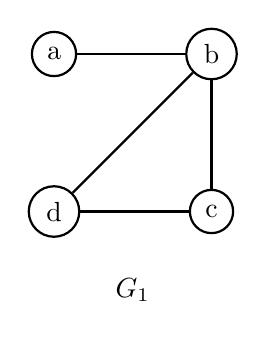
\begin{tikzpicture}
  \begin{scope}[every node/.style={circle,thick,draw}]
  \node (a) at (0,2) {a};
  \node (b) at (2,2) {b};
  \node (c) at (2,0) {c};
  \node (d) at (0,0) {d};
  \end{scope}
  \begin{scope}[every edge/.style={draw=black,thick}]
  \path (a) edge (b);
  \path (b) edge (c);
  \path (b) edge (d);
  \path (c) edge (d);
  \end{scope}
  \node () at (1,-1) {$G_1$};
  \end{tikzpicture}
  \hspace{1.5cm}
  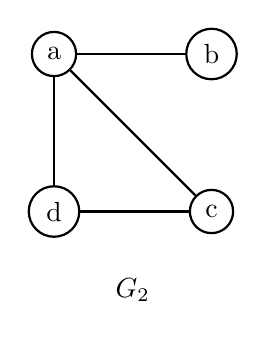
\begin{tikzpicture}
  \begin{scope}[every node/.style={circle,thick,draw}]
  \node (1) at (0,2) {a};
  \node (2) at (2,2) {b};
  \node (3) at (2,0) {c};
  \node (4) at (0,0) {d};
  \end{scope}
  \begin{scope}[every edge/.style={draw=black,thick}]
  \path (1) edge (2);
  \path (1) edge (3);
  \path (1) edge (4);
  \path (3) edge (4);
  \end{scope}
  \node () at (1,-1) {$G_2$};
  \end{tikzpicture}
  \caption{Nice pictures}
  \label{tikz:graphs}
\end{figure}


\begin{figure}
  \centering
  \begin{tikzpicture}[node distance=6cm]
  \node (a) [rect] {A Big Blue Block};
  \node (b) [oval, right of=a] {And His Oval Friend};
  \draw [line] (a) -- (b);
  \end{tikzpicture}
  \caption{Nice pictures}

\end{figure}


\chapter{Technology Review}
About seven to ten pages.
\begin{itemize}
\item Describe each of the technologies you used at a conceptual level. Standards, Database Model (e.g. MongoDB, CouchDB), XMl, WSDL, JSON, JAXP.
\item Use references (IEEE format, e.g. [1]), Books, Papers, URLs (timestamp) – sources should be authoritative.
\end{itemize}

\section{XML}
Here's some nicely formatted XML:
\begin{minted}{xml}
<this>
  <looks lookswhat="good">
    Good
  </looks>
</this>
\end{minted}

\chapter{System Design}
As many pages as needed.
\begin{itemize}
\item Architecture, UML etc. An overview of the different components of the system. Diagrams etc… Screen shots etc.
\end{itemize}

\begin{table}[h]
  \centering
  \begin{tabular}{x{2cm}p{3cm}}
    \toprule \\
    Column 1 & Column 2 \\
    \midrule \\
    Rows 2.1 & Row 2.2 \\
    \bottomrule
  \end{tabular}
  \caption{A table.}
  \label{table:mytable}
\end{table}

\chapter{System Evaluation}
As many pages as needed.
\begin{itemize}
\item Prove that your software is robust. How? Testing etc.
\item Use performance benchmarks (space and time) if algorithmic.
\item Measure the outcomes / outputs of your system / software against the objectives from the Introduction.
\item Highlight any limitations or opportuni-ties in your approach or technologies used.
\end{itemize}

\chapter{Conclusion}
About three pages.
\begin{appendices}
\chapter{Preamble \& Intro}
\begin{itemize}
\item \href{https://github.com/Ultan-Kearns/AppliedProject}{Link to my github}
\end{itemize}
\end{appendices}
\bibliographystyle{ieeetr}
\bibliography{bibliography}
\end{document}
